\documentclass[a4paper]{report}
\usepackage[utf8]{inputenc}
\usepackage[numbers]{natbib} % scientific references in the bibliography
\usepackage{hyperref}
\usepackage{graphicx}
%\usepackage{datetime}
\usepackage{color}
%\usepackage{microtype}
%\usepackage{draftwatermark}

%% Nicely format and linebreak URLs in the bibliography
%\usepackage{url}

%% Nicer formatting of figure captions.
%\usepackage[font=small,format=plain,labelfont=bf,up,textfont=it,up]{caption}

%\SetWatermarkScale{5}

%% Define a new 'leo' style for the package that will use a smaller font.
%\makeatletter
%\def\url@leostyle{%
%  \@ifundefined{selectfont}{\def\UrlFont{\sf}}{\def\UrlFont{\small\ttfamily}}}
%\makeatother
%% Now actually use the newly defined style.
%\urlstyle{leo}

%\newcommand{\hi}[1]{{\color{red}\tiny \em #1\/}\\}
\newcommand{\todo}[1]{\footnote{{\color{red} TODO: #1}}}

% ------------------------------------------------------------------------------
% Metadata
% ------------------------------------------------------------------------------
\title{Ontology Learning from Swedish Text}

\author{Jan Daniel Bothma}

% ------------------------------------------------------------------------------
% Document
% ------------------------------------------------------------------------------
\begin{document}

\maketitle

\begin{abstract}
Ontology learning is the process of analyzing text to construct an ontology which represents the meaning encoded in the text.
Many methods have been proposed and evaluated for extracting concepts, relations, hierarchies and axioms from text, particularly for the earlier stages of the process.
Open questions in this field include researching new methods; exploiting social, structured and collaboratively curated data; evaluating, comparing and combining methods; scaling to larger corpora; supporting various and cross-language corpora; supporting ongoing ontology development; and improving user interaction.
This thesis contributes a survey of high level requirements for application and ongoing research of ontology learning, and applies several existing methods to learn ontologies from Swedish text.
Result is TODO.
\end{abstract}	

\tableofcontents

\chapter{Introduction}
%ONE-SENT Ontology learning learning tools significantly speed up the knowledge extraction part of the Knowledge Engineering process. I'm going to investigate ontology learning from Swedish text.
%%UU-CHAP Motivation for the Project
%%UU-CHAP Background to the problem or system
%%"I am going to look at the following things"

By encoding semantic information about the world in a form that can be processed by computers, computers can provide better support in many tasks.
For example, the \emph{semantically enabled} IURISERVICE iFAQ database of legal questions and answers given by experienced Spanish judges, aims to support inexperienced judges in answering legal questions\cite{IURISERVICEPerformance2007}.
Important terms in the questions and answers are associated with their synonyms and the domain of law that they apply to.
When a question is entered to search for related question-answer pairs, the semantic information is used to improve the results over a plain text search, even when considering different forms of the words in the query.
The query is expanded to include exact matches, morphological variations\footnote{In the linguistic sense, such as \emph{car} to \emph{cars} for plurality}, and synonyms.
The similarity of the result questions to the query question is then calculated, considering the similarity of concepts and the grammatical structure of the questions, to provide the most-similar results to the user.
The semantic information is further used to provide suggestions of relevant legal cases whose decisions might have an impact on the issue at hand.

\section{Semantic Web}

By making semantic information available over the internet, many resources can be combined to support complex tasks involving many parties.
The Semantic Web\footnote{http://www.w3.org/2001/sw/} is the manifestation of this.
In a hypothetical example, Tim Berners-Lee et al. \footnote{Tim Berners-Lee, James Hendler and Ora Lassila. The Semantic Web. \emph{Scientific American}, 284(August), p.3863170-3863170 2001} describe a scenario where a brother and a sister try to book medical appointments for their mother with a nearby treatment centre available to their mother's health insurance policy, on dates that they can alternate driving their mother.
Information about their availability, the clinics (including treatments they offer and their schedules) and the insurance policy must be available to the computers involved in proposing a solution.
Furthermore, the meaning of this information, and how it relates to the other information involved in the computation, must be available.
For example, the computer must be able to distinguish between the treatment centre's postal address and their visiting address.
This information is encoded in ontologies and mappings between semantic entities in standardised formats such as OWL\cite{OWLOverview2004} to support this interoperability.

\section{Ontologies}

A commonly-cited definition of ontologies in the field of knowledge engineering is as \emph{``a formal, explicit specification of a shared conceptualization''} \cite{StuderEtAl1998KEPM}.
Here, a \emph{conceptualization} is the objects, concepts and relations between them, in an abstract view of the world intended for a particular purpose.
The conceptualization should be \emph{shared} within the context of its application.
The objective with this explicit specification is to allow computer agents to operate on this view of the world or for its integration in human-operated software.

Top level ontologies, domain ontologies

\section{Ontology Engineering}

stages of OE, ongoing process, facts change

place of OE w.r.t. information extraction, knowledge representation

place of ontology learning within OE

\section{Ontology Learning}

The automatic or semi-automatic construction of ontologies is called Ontology Learning \cite{Cimiano06}.
Ontology Learning commonly involves some combination of preprocesing, term extraction, concept formation, concept hierarchy induction, non-taxonomic relation learning, and axiom extraction.
Most approaches to these tasks are commonly mainly logical, statistical or linguistic in nature\cite{Wong11Survey}.
Such a categorisation is shown in Fig.~\ref{fig:tasktechout}.
\begin{figure}
  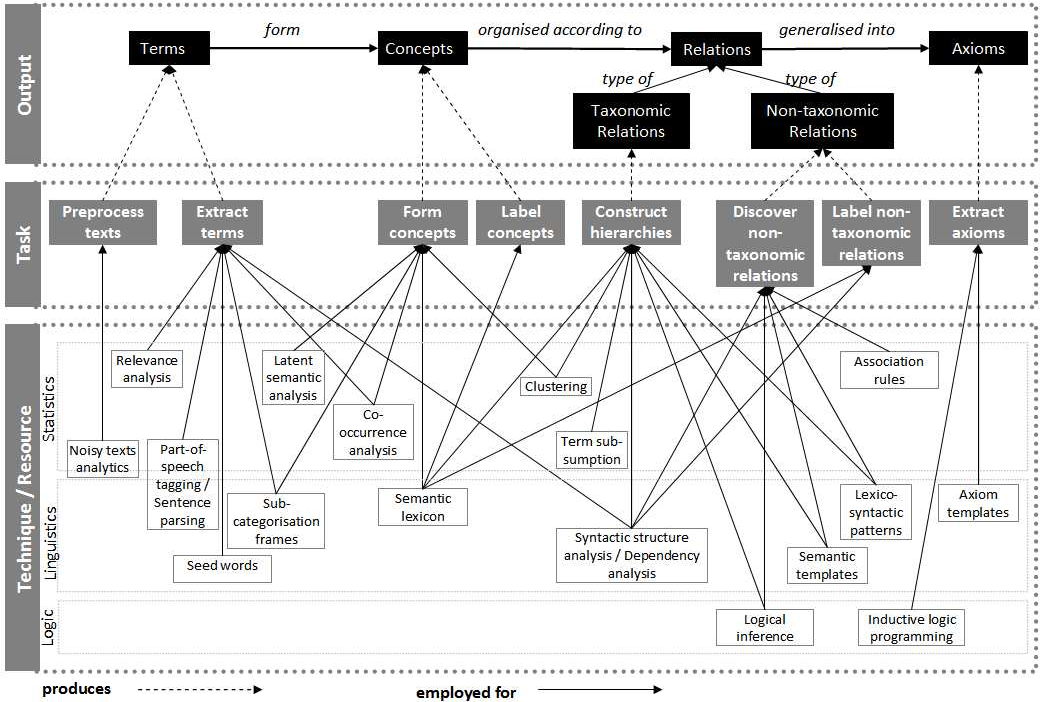
\includegraphics[width=\textwidth]{graphics/output-task-technique-WongLiuBennamoun.png}
  \caption{Tasks, techniques and outputs in ontology learning. Awaiting permission for reuse from \cite{Wong2009PhD}.}
  \label{fig:tasktechout}
\end{figure}
The task of \emph{ontology construction} is where ontology learning meets ontology engineering.
Ontology learning might produce an initial ontology used as a basis for further ontology development \cite{Voelkner2008Spanish}, or it can be used to suggest changes as part of an ongoing ontology engineering process.

Many methods for extracting the various ontology elements have been proposed and evaluated, often in comparison with other methods.
Preprocessing is mainly concerned with syntactic analysis of the corpora \todo{define corpora} and methods taken from the field of Natural Language Processing are applied.
The subsequent stages - concerned with \emph{semantic analysis} - 

\todo{give some examples of well-evaluated and newer techniques and their evaluation}

\section{Problem}
%ONE-SENT Hoewever, there is no Ontology Learning System for learning ontologies from Swedish text.

While blah many techniques for extracting terms and concepts have matured and have been evaluated against various competing techniques and in various settings, many areas of research are still somewhat unexplored.
Additionally, new technologies and on-line communities are providing new opportunities for supporting ontology learning.

Many existing methods rely on domain-specific models which need to be trained.
This training often involves manually annotated corpora which are time-consuming to produce, require domain expertise and aren't error-free.
There has been relatively little research in combining evidence from various languages.

\section{Objective}

given this background, the objectives of this thesis are

\begin{itemize}
  \item to provide a prototype system for learning domain ontologies from Swedish domain corpora
  \item to learn more about the tool framework needed to support application and ongoing research of Ontology Learning
\end{itemize}

\section{Research Questions}

We will fulfill these objectives by answering these research questions:

\begin{enumerate}
  \item{What are the general requirements for ontology learning research and application?}
  \item{How do common ontology learning methods need to be modified to extract ontologies from Swedish text?}
  \item{How do these modified methods perform compared to \todo{some baseline??? evaluation}?}
\end{enumerate}

\section{Approach}
%ONE-SENT

We expect many of the existing methods to work similarly well for Swedish as they do for English and other languages.
Intuitively, any method should work as well for Swedish as it does for English, as long as the assumptions behind it hold.
For example, term extraction based on the frequency of nouns should be very similar, but might be affected by word compounding in Swedish, which hardly occurs in English.

We will evaluate one or more existing approach for extracting terms, forming concepts, and extracting taxonomic and non-taxonomic relations on Swedish text with preprocessing tools for Swedish.


To address these questions, we will...

\begin{itemize}
  \item produce a list of requirements
  \item sketch an architecture
  \item implement a prototype system
    \begin{itemize}
      \item reusing as much as possible
      \item describing how techniques had to be modified to work for Swedish
    \end{itemize}
  \item evaluate somehow
\end{itemize}

\section{Delimitations}

Ontological Architecture is how an ontology is constructed to be most useful where it is applied \cite{OntArchChapter}. While flexibility to support architectural decisions was considered, this area was not thoroughly researched in this thesis.

The prototype is intended to elicit issues where the proposed requirements and architecture can be improved upon.
It is not intended to be the final platform implementation.

The implications of following one school of thought in meaning representation with regard to semantic parsing (e.g. Davidsonian \cite{DavidsonianSemantics}) over another have not been taken into account.
This factor is expected to introduce some bias in the knowledge extracted, but the lack of thorough investigation of its implications on the requirements discussed in this research is a limitation of this work.

\section{Report Structure}

The rest of this report will be structured as follows:

\chapter{Background}
%%UU-CHAP Overview of relevant research and development that is used in specifying the problem and obtaining and evaluating appropriate solutions.
%%ONE-SENT Many methods for the subtasks have been developed for other languages, and some have already been applied to Swedish, but they have not been combined and evaluated as a pipeline. Furthermore, none of the existing OL systems are suitable to be extended to Swedish, nor support the necessary evaluation approaches.
%%UU-REQ Awareness of relevant prior research and development literature
%% -- comment on its relevance. In what way _is_ it relevant and in what way is it _not_ relevant.
%%UU-REQ critical appraisal of that literature as a basis for the formulation of project objectives and the conduct of the project.
%% -- quality of the literature affects its bearing on the project. Note on the quality of an evaluation keeping in mind whether a plain olde eval would have been suitable in the first place - what's the objective of the publication?

This chapter reviews the state of Ontology Learning research.
We will discuss several end-to-end ontology learning systems which propose novel approaches to the problem, several approaches to particular ontology learning tasks.
Finally, shortcomings and suggested research areas identified in existing research will be summarized.

An interesting new approach is described in \cite{Poon2010OntoUSP}...
\begin{itemize}
  \item{input is dependency parse}
  \item{output is formulas representing classes, relations, clusters of those}
  \item{evaluation was based prepossessing with domain-trained syntactic parser}
\end{itemize}

\chapter{Method}
%UU-CHAP Methods and techniques required
%ONE-SENT By making X modifications to existing methods, we can improve on the baseline of Y.   We evaluate these methods in by Z. We might even evaluate our evaluation tools.
%%Philosophy of Approach - show you can pick out important ideas succinctly
%%Plan of Attack - show you approached the problem in a systematic way

\chapter{Realisation}
%UU-CHAP Implementation and formulation of the solution chosen
%ONE-SENT We implement a system that allows easy selection or combination of methods and their results, and allow the evaluation of these methods individually, in combination, and in pipeline.
%%Description of the work - details, so that others can follow what you did
%%  -> reproducibility

\section{Architecture and High Level Design}

In this chapter we will discuss the design and implementation of a prototype system for automatically or semi-automatically extracting a domain ontology from domain-specific corpora in the Swedish language.

\section{Preprocessing Swedish text}

\section{Term Extraction}

\section{Concept Formation}

\section{Concept Hierarchy}

\section{Relation Extraction}

\section{Ontology Construction}

Here we describe how the evidence from the various stages can be use to build an ontology ready for validation.


\chapter{Evaluation}
%%UU-REQ Evidence that the student has made a critical evaluation of the significance of the project outcomes, limitations of the results
%ONE-SENT We achieved results comparable to what was done with language Q in R. We can extract concepts and relations from Swedish text with evaluation metric S result of T.
%UU-CHAP Data collection and analysis where relevant, or testing of the solution of product.
%% Critical analysis of the results - show you know its limitations

\chapter{Conclusion}
%%UU-CHAP Conclusions reached and future enhancement or work that could be conducted to refine the system.
%%UU-REQ Strength of the conclusions reached, including the ability to provide a concise summary of the significance of the work and reflect on work practice and outcomes with the intent to improve performance in future projects.
% summarise introduction with detail from Solution and Evaluation

\chapter{Further Work}
%% show you know what’s missing


\clearpage
%\addcontentsline{toc}{chapter}{References}
%\renewcommand\bibname{References}

%\renewcommand{\refname}{}
%\chapter{References}
\bibliographystyle{unsrt}
\bibliography{report}

\end{document}
